



\section{\rebuttal{Missing Proofs}}
In this section, we will theoretically analyze UDS and other reweighting schemes to better understand when these approaches can perform well. We will first discuss our notation, then present our theoretical results, then discuss the intuitive explanations of these results, and finally, provide proofs of the theoretical results.

% \subsection{\rebuttal{Assumptions}}
% \label{app:notation}
% Let $\pi_\beta(\mathbf{a}|\bs)$ denote the behavior policy of the dataset. The dataset, $\mathcal{D}$ 
% is generated from the marginal state-action distribution of $\pi_\beta$, i.e., $\mathcal{D} \sim d^{\pi_\beta}(\bs) \pi_\beta(\mathbf{a}|\bs)$. We define $d^{\pi}_{\mathcal{D}}$ as the state marginal distribution introduced by the dataset $\mathcal{D}$ under $\pi$. For our analysis, we will abstract conservative offline RL algorithms into a generic constrained policy optimization problem~\citep{kumar2020conservative}:
% \begin{align}
% \label{eqn:generic_offline_rl}
%     \pi^*(\mathbf{a}|\bs) := \arg \max_{\pi}~~ \widehat{J}_{\mathcal{D}}(\pi) - \frac{\alpha}{1 - \gamma} D(\pi, \pi_\beta).
% \end{align}  
% $J_{\mathcal{D}}(\pi)$ denotes the average return of policy $\pi$ in the empirical MDP induced by the transitions in the dataset, and $D(\pi, \pi_\beta)$ denotes a divergence measure (e.g., KL-divergence~\citep{jaques2019way,wu2019behavior}, MMD distance~\citep{kumar2019stabilizing} or $D_{\text{CQL}}$~\citep{kumar2020conservative}) between the learned policy $\pi$ and the behavior policy $\pi_\beta$ computed in expectation over the marginal state-action distribution induced by the policy in the empirical MDP induced by the dataset:
% \begin{align*}
%     D(\pi, \pi_\beta) = \mathbb{E}_{\bs \sim \widehat{d}^{\pi}_\mathcal{D}}\left[ D(\pi(\cdot|\bs), \pi_\beta(\cdot|\bs) \right].
% \end{align*}
% Let $D_\text{CQL}(p, q)$ denote the following distance between two distributions $p(\bx)$ and $q(\bx)$ with equal support $\mathcal{X}$:
% \begin{equation*}
%     D_\text{CQL}(p, q) := \sum_{\bx \in \mathcal{X}} p(\bx) \left(\frac{p(\bx)}{q(\bx)} - 1 \right).
% \end{equation*}
% Unless otherwise mentioned, we will drop the subscript ``CQL'' from $D_\text{CQL}$ and use $D$ and $D_\text{CQL}$ interchangeably. Prior works~\citep{kumar2020conservative,yu2021conservative} have shown that the optimal policy $\pi^*$ that optimizes Equation~\ref{eqn:generic_offline_rl} attains a high probability safe-policy improvement guarantee, i.e., $J(\pi^*) \geq J(\pi_\beta) - \zeta$, where $\zeta$ is:
% \begin{align}
%     \label{eqn:single_task_guarantee}
%     \zeta =  \mathcal{O}\left(\frac{1}{(1 - \gamma)^2}\right) \mathbb{E}_{\bs \sim d^{\pi^*}_{\mathcal{D}}}\left[\sqrt{\frac{D_{\text{CQL}}(\pi^*, \pi_\beta)(\bs) + 1}{|\mathcal{D}(\bs)|}} \right] - \frac{\alpha}{1 - \gamma} D(\pi^*, \pi_\beta).
% \end{align}
% The first term in Equation~\ref{eqn:single_task_guarantee} corresponds to the decrease in performance due to sampling error and this term is high when the single-task optimal policy $\pi^*_i$ visits rarely observed states in the dataset $\mathcal{D}_i$ and/or when the divergence from the behavior policy $\pi_\beta$ is higher under the states visited by the single-task policy $\bs \sim d^{\pi^*_i}_{\mathcal{D}_i}$. We will show that UDS and CDS+UDS enjoy safe policy improvement. In our analysis, we assume $r(\bs, \mathbf{a}) \in [0, 1]$. Finally, as discussed in Section~\ref{sec:prelim}, let $\mathcal{D}^\mathrm{eff}_i$ denote the relabeled dataset for task $i$, which includes both $\mathcal{D}_i$ and the transitions from other tasks relabeled with a $0$ reward.

% To prove our theoretical results, following prior work~\citep{kumar2020conservative,yu2021conservative} we assume that the empirical rewards and dynamics concentrate towards their mean.
% \begin{assumption}
% \label{assumption:conc}
%     $\forall~ \bs, \mathbf{a}$, the following relationships hold with high probability, $\geq 1 - \delta$
%     \begin{equation*}
%         |\widehat{r}(\bs, \mathbf{a}) - r(\bs, \mathbf{a})| \leq \frac{C_{r, \delta}}{\sqrt{|\mathcal{D}(\bs, \mathbf{a})|}}, ~~~ ||\widehat{P}(\bs'|\bs, \mathbf{a}) - P(\bs'|\bs, \mathbf{a})||_{1} \leq \frac{C_{P, \delta}}{\sqrt{|\mathcal{D}(\bs, \mathbf{a})|}}.
%     \end{equation*}
% \end{assumption}
% Similar to prior work~\citep{kumar2020conservative,yu2021conservative}, we also make a coverage assumption, i.e., we assume that each state-action pair is observed in the dataset $\mathcal{D}$, but the rewards and transition dynamics are stochastic, so, the occurrence of each state-action pair does not trivially imply good performance. To relax this assumption, we can extend our analysis to function approximation (e.g., linear function approximation~\citep{duan2020minimax}), where such a coverage assumption is only required on all directions of the feature space, and not all state-action pairs. This would not significantly change the analysis, and hence we opt for the simple but, at the same time, an illustrative analysis in a tabular setting here.


\subsection{\rebuttal{Performance Guarantee for UDS}}
\label{proof:uds_proof}
We first restate Proposition~\ref{prop:uds_ours} below for convenience, and we then provide a proof of the result.
\begin{theorem}[\textbf{Policy improvement guarantee for UDS}; restated.] 
\label{prop:uds_ours_restated}
Let $\pi^*_\text{UDS}$ denote the policy learned by UDS, and let $\pi^\mathrm{eff}_\beta(\mathbf{a}|\bs)$ denote the behavior policy for the combined dataset $\mathcal{D}^\mathrm{eff}$. Then with high probability $\geq 1 - \delta$, $\pi^*_\text{UDS}$ is a safe policy improvement over $\pi_\beta^\mathrm{eff}$, i.e.,
\begin{align*}
& J(\pi^*_\text{UDS}) \geq J(\pi_\beta^\mathrm{eff}) - \zeta_\text{err} +  \underbrace{\frac{\alpha}{1 - \gamma} D(\pi^*_\text{UDS}, \pi^\mathrm{eff}_\beta)}_{\text{(c): policy improvement}},\\
 ~\text{where:~~}& \zeta_\text{err} = \underbrace{\frac{\sum_{\bs, \mathbf{a}} \left( \widehat{d}^{\behavior^\mathrm{eff}}(\bs, \mathbf{a}) - \widehat{d}^{\pi^*_\text{UDS}}(\bs, \mathbf{a})\right)  \cdot (1 - f(\bs, \mathbf{a})) \cdot r(\bs, \mathbf{a})}{1 - \gamma}}_{ \text{(a): reward bias}} \\
 &~~~~~~~+ \underbrace{\mathcal{O}\left(\frac{\gamma}{(1 - \gamma)^2}\right) \left[\sqrt{\frac{D_{\text{CQL}}(\pi^*_\text{UDS}, \pi^\mathrm{eff}_\beta)(\bs)}{|\mathcal{D}^\mathrm{eff}(\bs)|}} \right]}_{\text{(b): sampling error}},
\end{align*}
where we use the notation $f(\bs, \mathbf{a}) := \frac{|\mathcal{D}_\mathrm{L}(\bs, \mathbf{a})|}{|\mathcal{D}^\mathrm{eff} (\bs, \mathbf{a})|}$.
\end{theorem}

\begin{proof}
We start with the loss decomposition of the improvement of the learned policy relative to the behavior policy with the affine transformation $g$:  
\begin{align*}
    J(\pi) - J(\pi_\beta) := \underbrace{J(\pi) - \widehat{J}(\pi)}_{(i)} + \underbrace{\widehat{J}(\pi)  - \widehat{J}(\pi_\beta)}_{(ii)} + \underbrace{\widehat{J}(\pi_\beta) - {J}(\pi_\beta)}_{(iii)}.
\end{align*}

Now we will discuss how to bound each of the terms: terms (i) and (ii) correspond to the divergence between the empirical policy return and the actual return. While usually, this difference depends on the sampling error and distributional shift, in our case, it additionally depends on the reward bias induced on the unlabeled data and the transformation $g$. We first discuss the terms that contribute to this reward bias.

\paragraph{Bounding the reward bias.} Denote the effective reward of a particular transition $(\bs, \mathbf{a}, r, \bs') \in \mathcal{D}^\mathrm{eff}$, as $\widehat{r}^\mathrm{eff}$, which considers contributions from both the reward $\widehat{r}(\bs, \mathbf{a})$ observed in dataset $\mathcal{D}_\mathrm{L}$, and the contribution of $0$ reward from the relabeled dataset:
\begin{align}
\label{eqn:relabeled_reward}
    \widehat{r}^\mathrm{eff}(\bs, \mathbf{a}) = \frac{|\mathcal{D}(\bs, \mathbf{a})| \cdot \widehat{r}(\bs, \mathbf{a}) + |\mathcal{D}^\mathrm{eff}(\bs, \mathbf{a}) \setminus \mathcal{D}(\bs, \mathbf{a})| \cdot 0}{|\mathcal{D}^\mathrm{eff}(\bs,\mathbf{a})|}
\end{align}
Define $f(\bs, \mathbf{a}) := \frac{|\mathcal{D}(\bs, \mathbf{a})|}{|\mathcal{D}^\mathrm{eff}(\bs, \mathbf{a})|}$ for notation compactness. Equation~\ref{eqn:relabeled_reward} can then be used to derive the following difference against the true rewards:
\begin{align}
\label{eqn:upper_bound_reward_bias}
    \widehat{r}^\mathrm{eff}(\bs, \mathbf{a}) &- r(\bs, \mathbf{a}) = f(\bs, \mathbf{a}) \left( \widehat{r}(\bs, \mathbf{a}) - r(\bs, \mathbf{a}) \right) + (1 - f(\bs, \mathbf{a})) \cdot (0 - r(\bs, \mathbf{a})) \\
    &\leq f(\bs, \mathbf{a}) \cdot \frac{C_{r, \delta}}{\sqrt{|\mathcal{D}(\bs, \mathbf{a})|}} - (1 - f(\bs, \mathbf{a})) \cdot r(\bs, \mathbf{a}),
\end{align}
where the last step follows from the fact that the ground-truth reward $r(\bs, \mathbf{a}) \in [0, 1]$. Now, we lower bound the reward bias as follows:
\begin{align}
    \label{eqn:lower_bound_reward_bias}
        \widehat{r}^\mathrm{eff}(\bs, \mathbf{a}) + &- r(\bs, \mathbf{a}) = f(\bs, \mathbf{a}) \cdot \left(\widehat{r}(\bs, \mathbf{a}) - r(\bs, \mathbf{a}) \right) + (1 - f(\bs, \mathbf{a})) \cdot (- r(\bs, \mathbf{a})) \\
        &\geq - f(\bs, \mathbf{a}) \cdot \frac{C_{r, \delta}}{\sqrt{|\mathcal{D}(\bs, \mathbf{a})|}} - (1 - f(\bs, \mathbf{a})) \cdot r(\bs, \mathbf{a}), \nonumber
\end{align}
where the last step follows from the fact that $r(\bs, \mathbf{a}) \leq 1$.

\paragraph{Upper bounding $\widehat{J}(\pi) - J(\pi)$.} Next, using the upper and lower bounds on the reward bias, we now derive an upper bound on the difference between the value of a policy computed under the empirical MDP and the actual MDP. To compute this difference, we follow the following steps
\begin{align}
\label{eqn:decomposition}
    &\widehat{J}(\pi) - J(\pi) = \frac{1}{1 - \gamma} \sum_{\bs, \mathbf{a}} \left(\widehat{d}^\pi_{\mathcal{D}^\mathrm{eff}}(\bs) \pi(\mathbf{a}|\bs) \widehat{r}^\mathrm{eff}(\bs, \mathbf{a}) - d^\pi(\bs) \pi(\mathbf{a}|\bs) r(\bs, \mathbf{a})\right)\\ 
    &= \frac{1}{1 - \gamma} \underbrace{\sum_{\bs,\mathbf{a}} \widehat{d}^\pi_{\mathcal{D}^\mathrm{eff}}(\bs) \pi(\mathbf{a}|\bs) \left(\widehat{r}^\mathrm{eff}(\bs, \mathbf{a}) - r(\bs, \mathbf{a})\right)}_{:= \Delta_1} + \frac{1}{1 - \gamma} \underbrace{\sum_{\bs, \mathbf{a}}\left(\widehat{d}^\pi_{\mathcal{D}^\mathrm{eff}}(\bs) - d^\pi(\bs)\right) \pi(\mathbf{a}|\bs) r(\bs, \mathbf{a})}_{:= \Delta_2} \nonumber
\end{align}
Following \citet{kumar2020conservative} (Theorem 3.6), we can bound the second term $\Delta_2$ using:
\begin{align}
\label{eqn:delta_2_bound}
    \left|\Delta_2\right| \leq \frac{\gamma C_{P, \delta}}{1 - \gamma} \mathbb{E}_{\bs \sim \widehat{d}^\pi_{\mathcal{D}^\mathrm{eff}}(\bs)}\left[ \frac{\sqrt{|\mathcal{A}|}}{\sqrt{|\mathcal{D}^\mathrm{eff}(\bs)|}} \sqrt{ D(\policy, \widehat{\pi}^\mathrm{eff}_\beta)(\bs) + 1} \right].
\end{align}
To upper bound $\Delta_1$, we utilize the reward upper bound from Equation~\ref{eqn:upper_bound_reward_bias}:
\begin{align}
    \Delta_1 &= \sum_{\bs} \widehat{d}^\pi_{\mathcal{D}^\mathrm{eff}}(\bs) \left( \sum_{\mathbf{a}} \pi(\mathbf{a}|\bs) \left(\widehat{r}^\mathrm{eff}(\bs, \mathbf{a}) - r(\bs, \mathbf{a})\right) \right) \\
    &\leq \underbrace{\sum_\bs \widehat{d}^\pi_{\mathcal{D}^\mathrm{eff}}(\bs) \sum_{\mathbf{a}} f(\bs, \mathbf{a}) \frac{C_{r, \delta}}{\sqrt{|\mathcal{D}(\bs)|}} \frac{\pi(\mathbf{a}|\bs)}{\sqrt{\hatbehavior(\mathbf{a}|\bs)}}}_{\:= \Delta'_1} - \underbrace{\sum_{\bs, \mathbf{a}}  \widehat{d}^\pi_{\mathcal{D}^\mathrm{eff}}(\bs) \pi(\mathbf{a}|\bs) \left[ (1 - f(\bs, \mathbf{a})) \cdot r(\bs, \mathbf{a}) \right]}_{:=\Delta_4}.  
\end{align}
Combining the results so far, we obtain, for any policy $\pi$:
\begin{align}
\label{eqn:sampling_error_upper_bound}
    J(\pi) &\geq \widehat{J}(\pi) - \frac{|\Delta_2|}{1 - \gamma} - \frac{|\Delta_1'|}{1 - \gamma} + \frac{\Delta_4}{1 - \gamma}.
\end{align}

\paragraph{Lower bounding $\widehat{J}(\pi) - J(\pi)$.} To lower bound this quantity, we follow the step shown in Equation~\ref{eqn:decomposition}, and lower bound the term $\Delta_2$ by using the negative of the RHS of Equation~\ref{eqn:delta_2_bound}, and lower bound $\Delta_1$ by upper bounding its absolute value as shown below:
\begin{align}
    &\Delta_1 =  \sum_{\bs} \widehat{d}^\pi_{\mathcal{D}^\mathrm{eff}}(\bs) \left( \sum_{\mathbf{a}} \pi(\mathbf{a}|\bs) \left(\widehat{r}^\mathrm{eff}(\bs, \mathbf{a}) - r(\bs, \mathbf{a})\right) \right) \\
    &\geq \underbrace{\sum_\bs \widehat{d}^\pi_{\mathcal{D}^\mathrm{eff}}(\bs) \sum_{\mathbf{a}} f(\bs, \mathbf{a}) \frac{C_{r, \delta}}{\sqrt{|\mathcal{D}(\bs)|}} \frac{\pi(\mathbf{a}|\bs)}{\sqrt{\hatbehavior(\mathbf{a}|\bs)}}}_{\:= \Delta'_1} + \sum_{\bs} \widehat{d}^\pi_{\mathcal{D}^\mathrm{eff}}(\bs) \sum_{\mathbf{a}} \pi(\mathbf{a}|\bs) \cdot (1 - f(\bs, \mathbf{a})) r(\bs, \mathbf{a}).  
\end{align}
This gives rise to the complete lower bound:
\begin{align}
\label{eqn:sampling_error_lower_bound}
   \widehat{J}(\pi) &\geq J(\pi) - \frac{|\Delta_2|}{1 - \gamma} - \frac{1}{1-\gamma} \sum_{\bs, \mathbf{a}} \widehat{d}^\pi_{\mathcal{D}^\mathrm{eff}_i}(\bs) \pi(\mathbf{a}|\bs) (1 - f(\bs, \mathbf{a})) r(\bs, \mathbf{a})  -  \frac{\Delta'_1}{1 - \gamma}.
\end{align}

\paragraph{Policy improvement term (ii).} Finally, the missing piece that needs to be bounded is the policy improvement term (ii) in the decomposition of $J(\pi) - J(\pi_\beta)$. Utilizing the abstract form of offline RL, we note that term (ii) is lower bounded as:
\begin{align}
\label{eqn:lower_bound_on_improvement}
    \text{term (ii)} \geq \frac{\alpha}{1 - \gamma} D(\pi, \pi_\beta).
\end{align}

\paragraph{Putting it all together.} To obtain the final expression of Proposition~\ref{prop:uds_ours}, we put all the parts together, and include some simplifications to obtain the final expression. The bound we show is relative to the effective behavior policy $\pi^\mathrm{eff}_\beta$. Applying Equation~\ref{eqn:sampling_error_lower_bound} for term (i) on policy $\pi$, Equation~\ref{eqn:lower_bound_on_improvement} for term (ii), and Equation~\ref{eqn:sampling_error_upper_bound} for the behavior policy $\pi^\mathrm{eff}_\beta$, we obtain the following:
\begin{align*}
    &J(\pi) - J(\pi_\beta^\mathrm{eff}) = J(\pi) - \widehat{J}(\pi) + \widehat{J}(\pi) - \widehat{J}(\pi_\beta^\mathrm{eff}) + \widehat{J}(\pi_\beta^\mathrm{eff}) - J(\pi_\beta^\mathrm{eff})\\
    &\geq -\frac{2 \gamma C_{P, \delta}}{(1 - \gamma)^2} \mathbb{E}_{\bs \sim \widehat{d}^\pi_{\mathcal{D}^\mathrm{eff}}(\bs)}\left[ \frac{\sqrt{|\mathcal{A}|}}{\sqrt{|\mathcal{D}^\mathrm{eff}(\bs)|}} \sqrt{ D(\policy, \widehat{\pi}^\mathrm{eff}_\beta)(\bs) + 1} \right] - \frac{2 C_{r, \delta}}{1 - \gamma} \mathbb{E}_{\bs, \mathbf{a} \sim \widehat{d}^\pi_{\mathcal{D}^\mathrm{eff}}} \left[ \frac{f(\bs, \mathbf{a})}{\sqrt{|\mathcal{D}(\bs, \mathbf{a})|}} \right]\\
    &~~~~~~~- \frac{1}{1 - \gamma} {\left( \mathbb{E}_{\bs, \mathbf{a} \sim d^{\behavior^\mathrm{eff}}_{\mathcal{D}^\mathrm{eff}}}\left[\left(1 - f(\bs, \mathbf{a})\right) r(\bs, \mathbf{a}) \right] \right) } + \frac{1}{1 - \gamma} \mathbb{E}_{\bs, \mathbf{a} \sim \widehat{d}^\pi_{\mathcal{D}^\mathrm{eff}}} \left[ (1 - f(\bs, \mathbf{a})) \cdot r(\bs, \mathbf{a}) \right]\\
    &~~~~~~~~~~+ \frac{\alpha}{1 - \gamma} D(\pi, \pi_\beta^\mathrm{eff}).
\end{align*}
Note that in the second step above, we upper bound the quantities $\Delta_1'$ and $\Delta_2$ corresponding to $\pi_\beta^\mathrm{eff}$ with twice the expression for policy $\pi$. This is because the effective behavior policy $\pi^\mathrm{eff}_\beta$ consists of a mixture of the original behavior policy $\hatbehavior$ with the additional data, and thus the new effective dataset consists of the original dataset $\mathcal{D}_i$ as its part. Upper bounding it with twice the corresponding term for $\pi$ is a valid bound, though a bit looser, but this bound suffices for our interpretations. 

For our analysis purposes, we will define the suboptimality induced in the bound due to reward bias for a given $u$ and $v$ as:
\begin{align}
\label{eqn:reward_bias}
    &\mathrm{RewardBias}(\pi, \pi^\mathrm{eff}_\beta) \\
    &= -\frac{1}{1 - \gamma} \left[ \mathbb{E}_{\bs, \mathbf{a} \sim \widehat{d}^\pi_{\mathcal{D}^\mathrm{eff}}} \left[ (1 - f(\bs, \mathbf{a})) \cdot r(\bs, \mathbf{a}) \right] - \left(\mathbb{E}_{\bs, \mathbf{a} \sim d^{\behavior^\mathrm{eff}}_{\mathcal{D}^\mathrm{eff}}}\left[\left(1 - f(\bs, \mathbf{a})\right) r(\bs, \mathbf{a}) \right] \right) \right]
\end{align}
Thus, we obtain the desired bound in Proposition~\ref{prop:uds_ours}.
\end{proof}


\subsection{When is Reward Bias Small? Proof of Theorem \ref{prop:reward_bias_theorem}}
\label{sec:small_reward_bias}
Next, we wish to understand when the reward bias in Equation~\ref{eqn:reward_bias} is small. Concretely, we wish to search for effective behavior policies such that the dataset induced by them attains a small reward bias. Therefore we provide a proof for Theorem~\ref{prop:reward_bias_theorem} in this section.

\begin{proof}
We can express the reward bias as:
\begin{align*}
    \mathrm{RewardBias}(\pi, \pi^\mathrm{eff}_\beta) &:= - \frac{1}{1 - \gamma} \sum_{\bs, \mathbf{a}} \left(\widehat{d}^\pi_{\mathcal{D}^\mathrm{eff}}(\bs, \mathbf{a}) - \widehat{d}^{\behavior^\mathrm{eff}}_{\mathcal{D}^\mathrm{eff}}(\bs, \mathbf{a}) \right) \cdot (1 - f(\bs, \mathbf{a})) \cdot r(\bs, \mathbf{a}),
\end{align*}
Now, since our goal is to minimize the reward bias with respect to the effective behavior policy, we minimize the expression for suboptimality induced due to reward bias, shown above with respect to $\pi^\mathrm{eff}_\beta$. Before performing the differentiation step, we note the following simplification (we drop the $\mathcal{D}^\mathrm{eff}$ from the notation in $d^{\behavior^{\mathrm{eff}}}_{\mathcal{D}^\mathrm{eff}}$ to make the notation less cluttered below):
\begin{align}
    & \min_{\pi^\mathrm{eff}_\beta}~~  \mathrm{RewardBias}(\pi, \pi^\mathrm{eff}_\beta) \\
    & := \min_{\pi^\mathrm{eff}_\beta}~~ -\left(\widehat{J}(\pi) - \widehat{J}(\pi_\beta^\mathrm{eff}) \right) + \frac{1}{(1 - \gamma)} \sum_{\bs, \mathbf{a}} r(\bs, \mathbf{a}) f(\bs, \mathbf{a})  \left(\widehat{d}^\pi_{\mathcal{D}^\mathrm{eff}}(\bs, \mathbf{a}) - d^{\behavior^\mathrm{eff}}_{\mathcal{D}^\mathrm{eff}}(\bs, \mathbf{a}) \right) \nonumber\\
    & = \min_{\pi^\mathrm{eff}_\beta}~~ - \widehat{J}(\pi) + \widehat{J}(\pi^\mathrm{eff}_\beta) + \frac{1}{(1 - \gamma) |\mathcal{D}^\mathrm{eff}|}\sum_{\bs, \mathbf{a}} |\mathcal{D}(\bs, \mathbf{a})| r(\bs, \mathbf{a}) \left( \frac{\widehat{d}^\pi(\bs, \mathbf{a})}{\widehat{d}^{\pi_\beta^\mathrm{eff}}(\bs, \mathbf{a})} - 1 \right) \nonumber\\
    &= \min_{\pi^\mathrm{eff}_\beta}~~ \widehat{J}(\pi^\mathrm{eff}_\beta) +  \frac{1}{(1 - \gamma) |\mathcal{D}^\mathrm{eff}|}\sum_{\bs, \mathbf{a}} |\mathcal{D}(\bs, \mathbf{a})| r(\bs, \mathbf{a}) \left( \frac{\widehat{d}^\pi(\bs, \mathbf{a})}{\widehat{d}^{\pi_\beta^\mathrm{eff}}(\bs, \mathbf{a})} - 1 \right). \label{eq:final_Expr}
\end{align}
Now, since we can express the entire objective in Equation~\ref{eq:final_Expr} as a function of $\widehat{d}^{\behavior^\mathrm{eff}}$ since $\widehat{J}(\pi^\mathrm{eff}_\beta) = \sum_{\bs, \mathbf{a}} \widehat{d}^{\behavior^\mathrm{eff}}(\bs, \mathbf{a}) r(\bs, \mathbf{a})$, we can compute and set the derivative of Equation~\ref{eq:final_Expr} with respect to $\widehat{d}^{\behavior^\mathrm{eff}}(\bs, \mathbf{a})$ as 0 while adding down the constraints that pertain to the validity of $\pi$. This gives us:
\begin{equation*}
    \widehat{d}^\pi(\bs, \mathbf{a}) \propto \sqrt{\frac{{|\mathcal{D}(\bs , \mathbf{a})| \cdot \widehat{d}^\pi(\bs, \mathbf{a})}}{|\mathcal{D}^\mathrm{eff}|}}. 
\end{equation*}
Substituting $|\mathcal{D}(\bs,\mathbf{a})| = \widehat{d}_\mathrm{L}(\bs, \mathbf{a}) \cdot |\mathcal{D}_\mathrm{L}|$ we obtain the desired result.
\end{proof}


\subsection{When is The Bound in Theorem~\ref{prop:uds_ours} Tightest?: Proof of Theorem~\ref{thm:with_all_sources}}
\label{proof:all_sources}
In this section, we will formally state and provide a proof for Theorem~\ref{thm:with_all_sources}. To prove this result, we first compute an upper bound on the error terms (a) and (b) in Theorem~\ref{thm:with_all_sources}, and show that the optimized distribution shown in Theorem~\ref{thm:with_all_sources} emerges as a direct consequence of optimizing this bound. To begin, we compute a different upper bound on sampling error than the one used in Theorem~\ref{thm:with_all_sources}. Defining the sampling error for a policy $\pi$ as the difference in return in the original and the empirical MDPs $\Delta_\text{sampling} = \widehat{J}(\pi) - J(\pi)$, we obtain the following Lemma:

\begin{lemma}[Upper bound on sampling error in terms of $\widehat{d}^\pi(\bs, \mathbf{a})$]
We can upper bound sampling error term as follows: 
\begin{align}
\label{eqn:upper_bound_on_sampling}
    \Delta_\text{sampling} \leq \frac{\gamma C_{P, \delta}}{(1 - \gamma)^2 \sqrt{|\mathcal{D}|}} \sum_{\bs, \mathbf{a}} \frac{\widehat{d}^\pi(\bs, \mathbf{a})}{\sqrt{\widehat{d}^{\pi_\beta^\mathrm{eff}}(\bs, \mathbf{a})}}.
\end{align}
\end{lemma}
\begin{proof}
For this proof, we will derive a bound on the sampling error, starting from scratch, but this time only in terms of the state-action marginals: 
\begin{align*}
    \Delta_{\text{sampling}} &= \frac{1}{1 - \gamma} \sum_{\bs, \mathbf{a}} \left( \widehat{d}^\pi(\bs, \mathbf{a}) - d^\pi(\bs, \mathbf{a}) \right) \cdot r(\bs, \mathbf{a})
\end{align*}
Note that we can bound $\Delta_\text{sampling}$ by upper bounding the total variation between marginal state-action distributions in the empirical and actual MDPs, i.e., $\vert\vert \widehat{d}^\policy - d^\policy \vert\vert_1$, since $|r_M(\bs, \mathbf{a})| \leq R_{\max}$. and hence we bound the second term effectively. Our analysis is similar to \citet{achiam2017constrained}. Define, $G = (I - \gamma P^{\policy})^{-1}$ and $\mathbf{a}r{G} = (I - \gamma \widehat{P}^\policy)^{-1}$. Then,
\begin{equation*}
    \widehat{d}^\policy - d^\policy = (1 - \gamma) (\mathbf{a}r{G} - G) \rho,
\end{equation*}
where $\rho(\bs)$ is the initial state distribution. Then we can use the derivation in proof of Theorem 3.6 in \citet{kumar2020conservative} or Equation 21 from \citet{achiam2017constrained}, to bound this difference as
\begin{align*}
    \vert\vert d^\policy - \widehat{d}^\policy||_{1} &\leq \frac{\gamma}{1 - \gamma} \sum_{\bs} \widehat{d}^\policy(\bs) \frac{C_{P, \delta}}{\sqrt{|\mathcal{D}(\bs)|}} \sum_{\mathbf{a}}  \frac{\policy(\mathbf{a}|\bs)}{\sqrt{\behavior(\mathbf{a}|\bs)}}\\
    &\leq \frac{\gamma C_{P, \delta}}{(1 - \gamma) \sqrt{|\mathcal{D}|}} \sum_{\bs, \mathbf{a}} \frac{\widehat{d}^\pi(\bs, \mathbf{a})}{\sqrt{\widehat{d}^{\pi_\beta^\mathrm{eff}}(\bs, \mathbf{a})}}.
\end{align*}
Thus the sampling error can be bounded by:
\begin{align*}
    \Delta_\text{sampling} \leq \frac{\gamma C_{P, \delta}}{(1 - \gamma)^2 \sqrt{|\mathcal{D}|}} \sum_{\bs, \mathbf{a}} \frac{\widehat{d}^\pi(\bs, \mathbf{a})}{\sqrt{\widehat{d}^{\pi_\beta^\mathrm{eff}}(\bs, \mathbf{a})}},
\end{align*}
which proves the lemma.
\end{proof}

\begin{theorem}[\textbf{Optimized reweighting unlabeled data}]
\label{thm:with_all_sources_restated}
The optimal effective behavior policy that maximizes a lower bound on $J(\pi^\mathrm{eff}_\beta) - \left[(a) + (b) \right]$ in Theorem~\ref{prop:uds_ours} satisfies: $d^{\widehat{\pi}_\beta^\mathrm{eff}}(\bs, \mathbf{a}) = p^*(\bs, \mathbf{a})$, where,
\begin{align*}
    p^* = \arg\min_{p \in \Delta^{|\mathcal{S}||\mathcal{A}|}}&~ \sum_{\bs, \mathbf{a}} C_1 \frac{\widehat{d}^\pi(\bs, \mathbf{a})}{\sqrt{p(\bs, \mathbf{a})}} + C_2 |d_\mathrm{L}(\bs, \mathbf{a})| \frac{\widehat{d}^\pi(\bs, \mathbf{a})}{p(\bs, \mathbf{a})}, 
\end{align*}
where $C_1$ and $C_2$ are universal positive constants that depend on the sizes of the labeled and unlabeled datasets are shown in Equation~\ref{eqn:c1_c2}.  
\end{theorem}

\begin{proof}
To prove this result, we will first simplify the expression containing all terms except the policy imnprovement term in Theorem~\ref{thm:with_all_sources}, so that we can then maximize the bound to obtain the statement of our theoretical statement. 
\begin{align*}
    (\bullet) &:= J(\pi^\mathrm{eff}_\beta) - \left[(a) + (b)\right] \geq\\ 
    &  J(\pi^\mathrm{eff}_\beta) + \frac{1}{1 - \gamma} \sum_{\bs, \mathbf{a}} \left(\widehat{d}^\pi(\bs, \mathbf{a}) - \widehat{d}^{\behavior^\mathrm{eff}}(\bs, \mathbf{a}) \right) \cdot (1 - f(\bs, \mathbf{a})) \cdot r(\bs, \mathbf{a}) - \Delta_\text{sampling}\\
    & \geq J(\pi^\mathrm{eff}_\beta) + \frac{1}{1 - \gamma} \sum_{\bs, \mathbf{a}} \left(\widehat{d}^\pi(\bs, \mathbf{a}) - \widehat{d}^{\behavior^\mathrm{eff}}(\bs, \mathbf{a}) \right) \cdot (1 - f(\bs, \mathbf{a})) \cdot r(\bs, \mathbf{a}) \\
    & ~~~~~~~~~~~~~~~~~~~~ - \frac{\gamma C_{P, \delta}}{(1 - \gamma)^2 \sqrt{|\mathcal{D}_\mathrm{eff}}|} \sum_{\bs, \mathbf{a}} \frac{\widehat{d}^\pi(\bs, \mathbf{a})}{\sqrt{\widehat{d}^{\pi_\beta^\mathrm{eff}}(\bs, \mathbf{a})}} 
\end{align*}
First of all we can lower bound, $J(\pi^\mathrm{eff}_\beta)$ in terms of the return of $\pi^\mathrm{eff}_\beta)$ in the empirical MDP induced by the dataset $\mathcal{D}_\mathrm{eff}$ and an irreducible sampling error term, that grows as $\mathcal{O}\left(\sqrt{1/{|\mathcal{D}^\mathrm{eff}|}}\right)$ and does not depend on the distribution of state-action pairs in the effective dataset, $\widehat{d}^{\pi_\beta^\mathrm{eff}}(\bs, \mathbf{a})$, but only depends on its size. Using this result, and by performing algebraic manipulation, we can further simplify this as:
\begin{align*}
    (\bullet) &\geq \cancel{\widehat{J}(\pi^\mathrm{eff}_\beta)} + \widehat{J}(\pi) - \cancel{\widehat{J}(\pi^\mathrm{eff}_\beta)} - \frac{\sum_{\bs, \mathbf{a}} |\mathcal{D}(\bs, \mathbf{a})| r(\bs, \mathbf{a}) \left( \frac{\widehat{d}^\pi(\bs, \mathbf{a})}{\widehat{d}^{\pi_\beta^\mathrm{eff}}(\bs, \mathbf{a})} - 1 \right)}{(1 - \gamma) |\mathcal{D}^\mathrm{eff}|} \\
    & ~~~~~~~~~~~~~~~~~~~~~~~~~~~~~ - \frac{\gamma C_{P, \delta}}{(1 - \gamma)^2 \sqrt{|\mathcal{D}_\mathrm{eff}}|} \sum_{\bs, \mathbf{a}} \frac{\widehat{d}^\pi(\bs, \mathbf{a})}{\sqrt{\widehat{d}^{\pi_\beta^\mathrm{eff}}(\bs, \mathbf{a})}} + \mathcal{O}\left(\sqrt{\frac{1}{|\mathcal{D}^\mathrm{eff}|}}\right)\\
    & \geq \widehat{J}(\pi) - \frac{1}{(1 - \gamma) |\mathcal{D}^\mathrm{eff}|}\sum_{\bs, \mathbf{a}} |\mathcal{D}(\bs, \mathbf{a})| r(\bs, \mathbf{a}) \left( \frac{\widehat{d}^\pi(\bs, \mathbf{a})}{\widehat{d}^{\pi_\beta^\mathrm{eff}}(\bs, \mathbf{a})} - 1 \right)\\
    & ~~~~~~~~~~~~~~~~~~~~~~~~~~~~~ - \frac{\gamma C_{P, \delta}}{(1 - \gamma)^2 \sqrt{|\mathcal{D}_\mathrm{eff}}|} \sum_{\bs, \mathbf{a}} \frac{\widehat{d}^\pi(\bs, \mathbf{a})}{\sqrt{\widehat{d}^{\pi_\beta^\mathrm{eff}}(\bs, \mathbf{a})}} + \mathcal{O}\left(\sqrt{\frac{1}{|\mathcal{D}^\mathrm{eff}|}}\right)\\
    & \geq \widehat{J}(\pi) - \frac{1}{(1 - \gamma) |\mathcal{D}^\mathrm{eff}|}\sum_{\bs, \mathbf{a}} |\mathcal{D}(\bs, \mathbf{a})| \left( \frac{\widehat{d}^\pi(\bs, \mathbf{a})}{\widehat{d}^{\pi_\beta^\mathrm{eff}}(\bs, \mathbf{a})} - 1 \right) \\ 
    & ~~~~~~~~~~~~~~~~~~~~~~~~~~~~~ - \frac{\gamma C_{P, \delta}}{(1 - \gamma)^2 \sqrt{|\mathcal{D}_\mathrm{eff}}|} \sum_{\bs, \mathbf{a}} \frac{\widehat{d}^\pi(\bs, \mathbf{a})}{\sqrt{\widehat{d}^{\pi_\beta^\mathrm{eff}}(\bs, \mathbf{a})}} + \mathcal{O}\left(\sqrt{\frac{1}{|\mathcal{D}^\mathrm{eff}|}}\right),
\end{align*}
where the last inequality follows from the fact that $|r(\bs, \mathbf{a})| \leq 1$. Since $|\mathcal{D}^\mathrm{eff}|$ and $\widehat{d}^{\pi_\beta^\mathrm{eff}}$ are decoupled (one is the distribution; other is the size of the dataset), we can optimize over each of them independently, and hence, we find that the distribution that optimizes this bound is given by:
\begin{align*}
    p^* = \arg\min_{p \in \Delta^{|\mathcal{S}||\mathcal{A}|}}&~ \sum_{\bs, \mathbf{a}} C_1 \frac{\widehat{d}^\pi(\bs, \mathbf{a})}{\sqrt{p(\bs, \mathbf{a})}} + C_2 |d_\mathrm{L}(\bs, \mathbf{a})| \frac{\widehat{d}^\pi(\bs, \mathbf{a})}{p(\bs, \mathbf{a})}, 
\end{align*}
where:
\begin{align}
\label{eqn:c1_c2}
    C_2 &:= \frac{|\mathcal{D}_\mathrm{L}|}{ (1 - \gamma) |\mathcal{D}_\mathrm{eff}|}, ~~~~~~~~ C_1 :=  \frac{\gamma C_{P, \delta}}{(1 - \gamma)^2 \sqrt{|\mathcal{D}_\mathrm{eff}}|}.
\end{align}
This proves Theorem~\ref{thm:with_all_sources}.
\end{proof}









\section{\rebuttal{Additional Empirical Analysis}}
\label{app:empirical_analysis}

\rebuttal{In this section, we perform an empirical study on the Meta-World domain to better understand the reason that UDS and CDS+UDS work well. Our theoretical analysis suggests that UDS will help the most on domains with limited data or narrow coverage or low data quality. To test these conditions in practice, we perform empirical analysis on two domains as follows.

\subsection{\rebuttal{Meta-World Domains}}
\label{app:mw_analysis}

\begin{table*}[t!]
\centering
\resizebox{\textwidth}{!}{\begin{tabular}{l|l|r|r|r}
\toprule
\textbf{Environment} & \textbf{Dataset type / size} & \textbf{CDS+UDS} & \textbf{UDS} & No Sharing\\
\midrule
& expert / 2k transitions & \textbf{67.6\%} & 58.8\% & 31.3\%\\
Meta-World door open & medium / 2k transitions & 67.3\% & \textbf{74.2\%} & 27.6\%\\
& medium-replay / 152k transitions & \textbf{30.0\%} & 0.0\% & 14.8\%\\
\bottomrule
\end{tabular}}
\caption{\footnotesize \rebuttal{We perform an empirical analysis on the Meta-World \texttt{door open} task where we use varying data quality and dataset size target task \texttt{door open}. We share the same dataset from the other three tasks in the multi-task Meta-World environment, \texttt{door close}, \texttt{drawer open} and \texttt{drawer close} to the target task. The numbers are averaged over three random seeds. CDS+UDS and UDS are able to outperform No Sharing in most of the settings except that UDS fails to achieve non-zero success rate in the medium-replay dataset with a large number of transitions. Such results suggest that CDS+UDS and UDS are robust to the data quality of the target task and work the best in settings where the target task has limited data.}}
\label{tbl:analysis}
\normalsize
\end{table*}

We first choose the \texttt{door open} task with three different combinations of dataset size and data quality of the task-specific data with reward labels:
\begin{itemize}
    \item 2k transitions with the expert-level performance (i.e. \textbf{high-quality data with limited sample size and narrow coverage})
    \item 2k transitions with medium-level performance (i.e. \textbf{medium-quality data with limited sample size and narrow coverage})
    \item a medium-replay dataset with 152k transitions (i.e. \textbf{medium-quality data with sufficient sample size and broad coverage}).
\end{itemize}
 We share the same data from the other three tasks, \texttt{door close}, \texttt{drawer open} and \texttt{drawer close} as in Table~\ref{tbl:gym}. As shown in Table~\ref{tbl:analysis}, both UDS and CDS+UDS are able to outperform No Sharing in the three settings, suggesting that increasing the coverage of the offline data as suggested by our theory does lead to performance boost in wherever we have limited good-quality data (expert), limited medium-quality data (medium) and abundant medium-quality data (medium-replay). It’s worth noting that UDS and CDS+UDS significantly outperform No Sharing in the limited expert and medium data setting whereas in the medium-replay setting with broader coverage, CDS+UDS outperforms No sharing but UDS fails to achieve non-zero success rate. Such results suggest that UDS and CDS+UDS can yield greater benefit when the target task doesn’t have sufficient data and the number of relabeled data is large. The fact that UDS is unable to learn on medium-replay datasets also suggests that data sharing without rewards is less useful in settings where the coverage of the labeled offline data is already quite broad.}

\subsection{\rebuttal{Ablation: Dataset Size}}
\label{app:unlabeled_dataset_size_analysis}

\begin{table*}[t!]
\centering
\scriptsize
\resizebox{\textwidth}{!}{\begin{tabular}{l|l|l|rr|r}
\toprule
 \textbf{Environment} & \textbf{Labeled dataset type / size} & \textbf{Unlabeled dataset type / size}   & \textbf{CDS+UDS}   & \textbf{UDS}          & \textbf{Sharing All (oracle)} \\
 \midrule
 & random / 10k transitions & expert / 10k transitions  & \textbf{10.1} & 10.0 & 71.9\\
 D4RL hopper & random / 10k transitions & expert / 100k transitions  & \textbf{105.8} & 81.8 & 96.3\\
& random / 10k transitions & expert / 1M transitions  & \textbf{102.3} & 97.0 & 102.8\\

\bottomrule
\end{tabular}}
\caption{\footnotesize Ablation study on the unlabeled dataset size ranging from 10k to 1M transitions in the single-task hopper domain. We bold the best method without true reward relabeling.}
\label{tbl:hopper_ablation}
\normalsize
\end{table*}

Following the discussion in Section~\ref{sec:uds_empirical_analysis}, we further study the setting where relabeled data has higher quality than the labeled data in the single-task hopper task by varying the amount of unlabeled data within the range of (10k, 100k, 1M) transitions. We pick the case where labeled data is random and unlabeled data is expert for such ablation study. As shown in Table~\ref{tbl:hopper_ablation}, as the unlabeled (expert) dataset size decreases, the result of UDS drops significantly whereas Sharing All retains a reasonable level of performance. This ablation suggests that as the effective dataset size decreases, the benefit of reducing sampling error is reduced and no longer able to outweigh the reward bias as indicated in our theoretical analysis. Moreover, Table~\ref{tbl:hopper_ablation} also suggests that, in the setting with medium unlabeled dataset size (100k transitions), CDS+UDS is able to prevent the performance drop as seen in UDS and even outperforms Sharing All. However, CDS+UDS cannot successfully tackle the case where there are only 10k unlabeled transitions, suggesting that the reward bias optimized by CDS+UDS is still detrimental in the limited unlabeled data regime.

\subsection{\final{Comparison to Reward-Learning Methods}}
\label{app:reward_learning_ablation}

\final{We performed an ablation that varies the labeled data size (10k \& 20k transitions) and quality (expert / random) for reward learning methods on D4RL hopper, with unlabeled data being 1M \texttt{hopper-medium} transitions.}
\begin{table*}[t!]
\centering
\footnotesize
\resizebox{\textwidth}{!}{\begin{tabular}{l|l|l|rrr}
\toprule
\vspace{-0.08cm}
 \textbf{Env} & \textbf{Labeled dataset type / size} & \textbf{Unlabeled dataset type / size}  & \textbf{CDS+UDS}   & \textbf{UDS}          & \textbf{Reward Pred.} \\
 \midrule
 & expert / 10k transitions & medium / 1M transitions & \textbf{78.3}$\pm$ 5.4 & 64.4$\pm$11.7 & 51.7 $\pm$8.4\\
  & expert / 20k transitions & medium / 1M transitions & 95.5$\pm$5.4 & \textbf{99.2}$\pm$3.1 & 96.7$\pm$3.6\\
 hopper & random / 10k transitions & medium / 1M transitions & \textbf{65.8}$\pm$11.3  & 51.9$\pm$2.4 & 33.4$\pm$5.4\\
 \vspace{-0.08cm}
& random / 20k transitions &medium / 1M transitions  & \textbf{69.1}$\pm$4.8 & 59.9$\pm$5.6 & 47.5$\pm$5.9\\
\bottomrule
\end{tabular}}
% \vspace{-0.4cm}
% \caption{\scriptsize Eval of COMBO, CQL + MBPO, and MOReL on generalization tasks.}
% \caption{}
\caption{\footnotesize Ablation study on comparisons between CDS+UDS/UDS and Reward Predictor with varying labeled dataset size and quality in the single-task hopper domain. We bold the best method.}
\label{tab:reward}
\normalsize
\vspace{-0.2cm}
\end{table*}
\final{Observe on the right, as expected, reward learning performs better with more labeled data. Furthermore, while reward learning works well when labeled data is high quality, it fails to perform well when labeled data is of low quality, potentially due to the bias in reward prediction. UDS and CDS+UDS are less sensitive to labeled data quality/size.}

\subsection{\rebuttal{Takeaways from the empirical analysis}}

Given our empirical analysis in Table~\ref{tbl:single_task_analysis}, Table~\ref{tbl:analysis}, Table~\ref{tbl:hopper_ablation} and Table~\ref{tab:reward}, we summarize the applicability of UDS / CDS+UDS under different scenarios for practitioners in Figure~\ref{fig:treeplot} below.

\begin{figure}[ht]
    \centering
    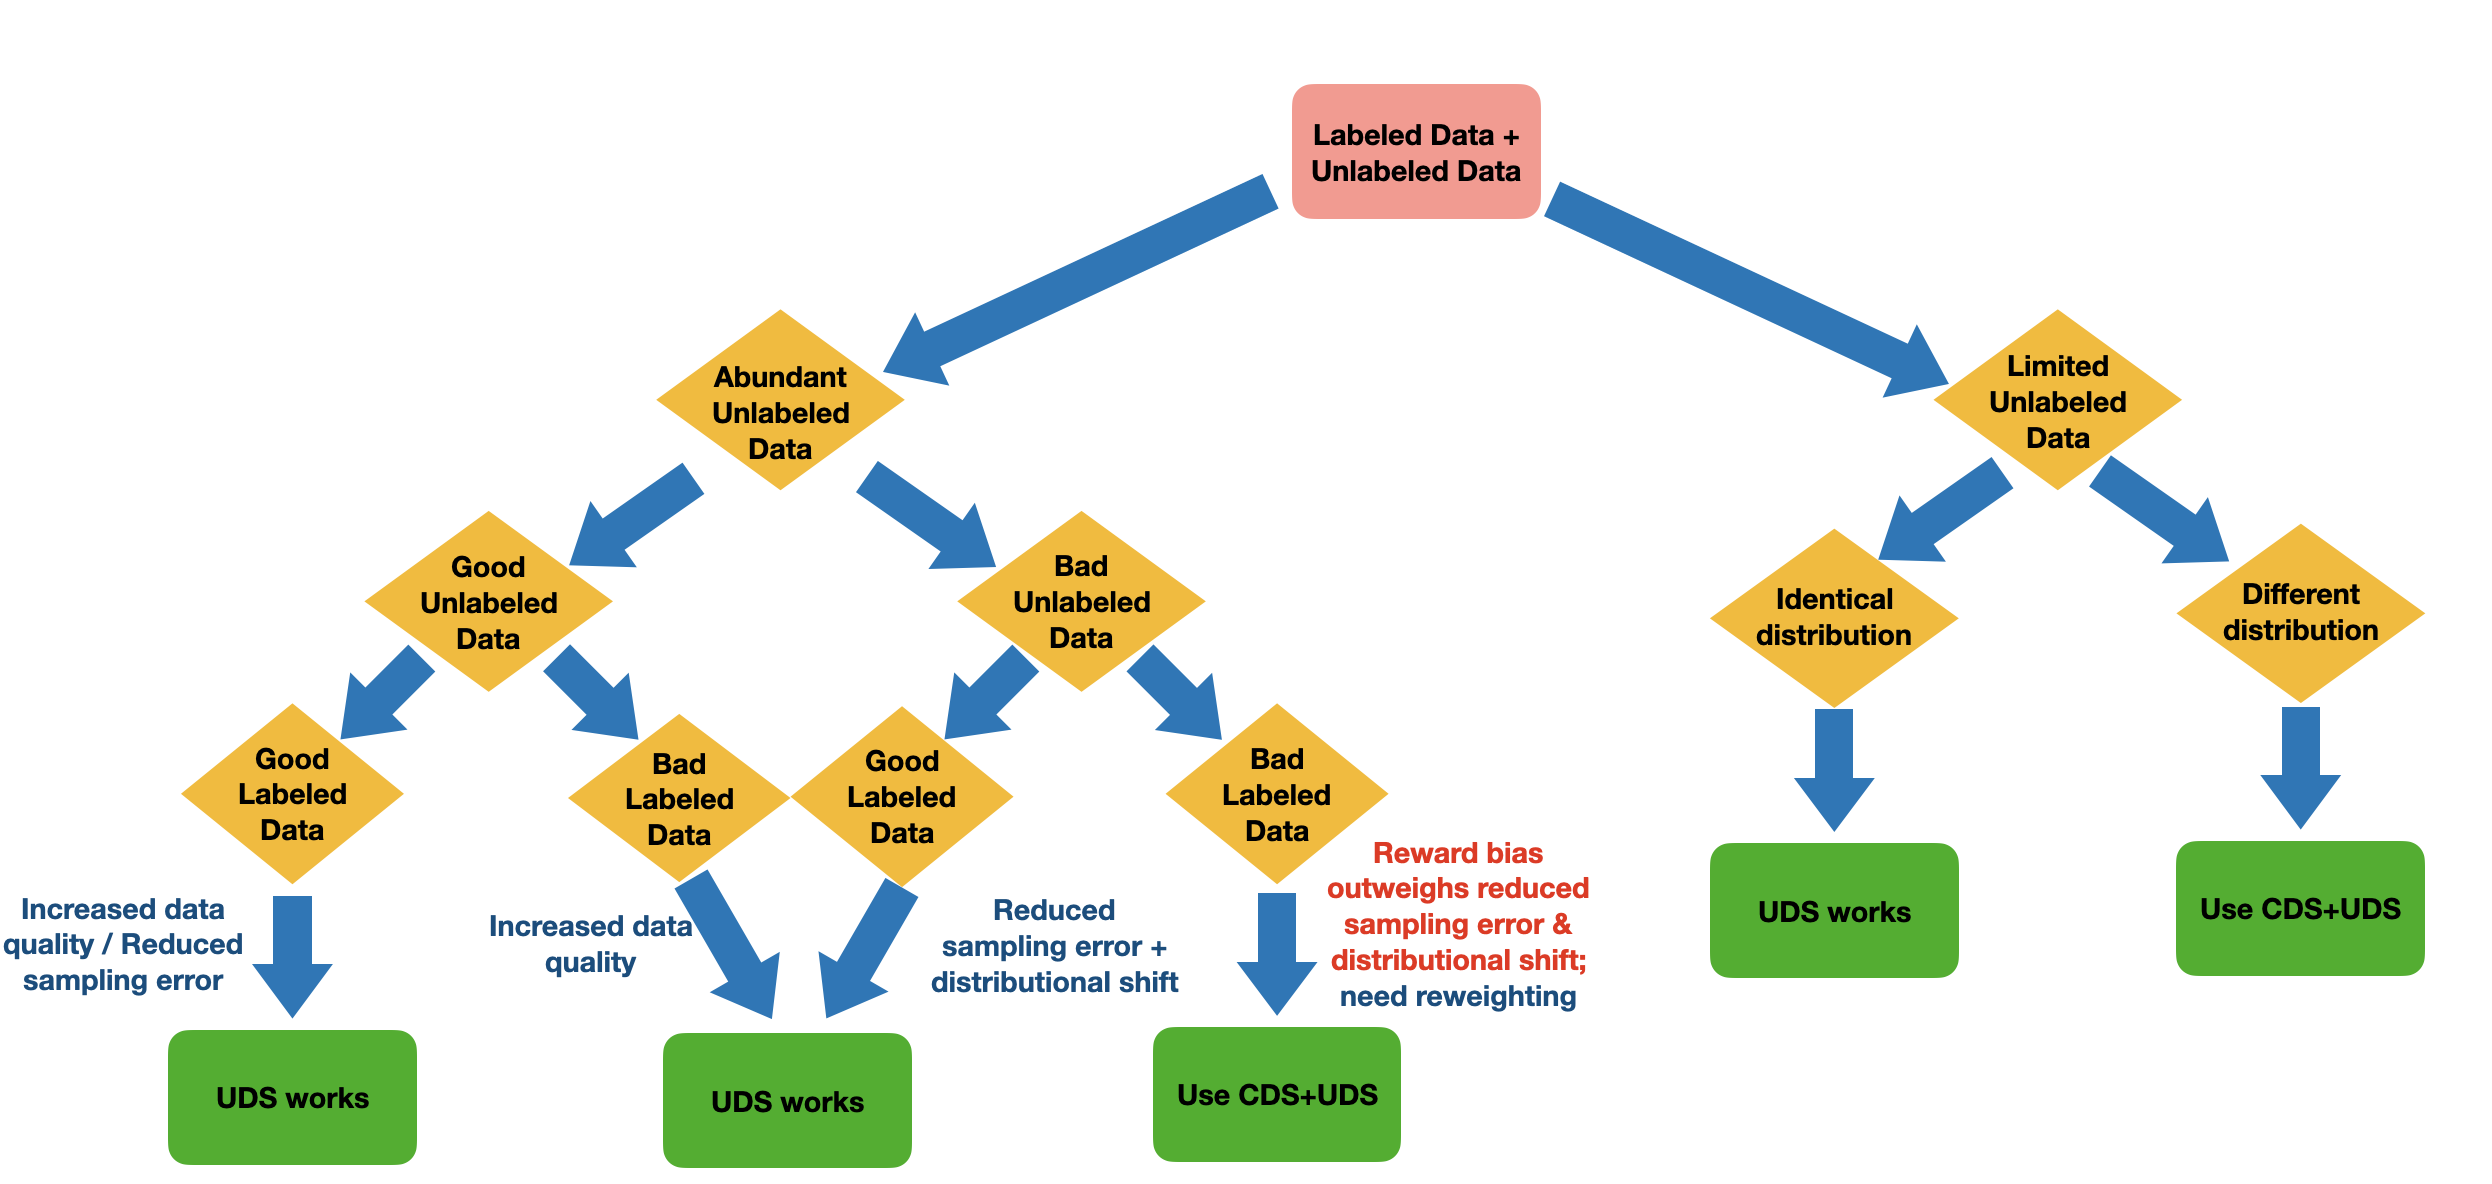
\includegraphics[width=0.95\textwidth]{chapters/uds/tree_plot.png}
    \vspace{-0.33cm}
    \caption{\footnotesize  A tree plot that illustrates under which conditions a practitioner should run UDS over apply the optimized reweighting scheme on top of UDS.}
    \vspace{-0.2cm}
    \label{fig:treeplot}
\end{figure}


\section{Additional Details About Data Quality}
\label{app:data_quality}

\begin{table*}[t!]
\centering
\resizebox{0.7\textwidth}{!}{\begin{tabular}{l|l|r}
\toprule
\textbf{Environment} & \textbf{Tasks} & \textbf{Oracle Success Rate of the Shared data}\\
\midrule
&drawer open & 47.4\%\\
& door close & 99.2\%\\
Meta-World& drawer open & 0.1\%\\
& drawer close & 91.6\%\%\\
& \CC \textbf{average} & \CC 59.5\%\\
\midrule
 & medium maze (3 tasks) average  &  4.3\% \\
AntMaze  & large maze (7 tasks) average  & 1.6\% \\
\bottomrule
\end{tabular}}
\caption{\footnotesize Success rate of the data shared from other tasks to the target task determined by the ground-truth multi-task reward function.}
\label{tbl:data_quality}
\normalsize
\end{table*}

We present the success rate of the data shared from other tasks to the target task computed by the oracle multi-task reward function in both the multi-task Meta-World and AntMaze domains in Table~\ref{tbl:data_quality}. Note that the success rate of \texttt{drawer close} and \texttt{door close} are particularly high since for other tasks, the drawer / door is initialized to be closed and therefore the success rate of other task data for these two tasks are almost 100\% as defined by the success condition in the public Meta-World repo. Apart from these two particularly high success rates, the success rates of the shared data are consistently above 0\% across all tasks in both domains. This fact suggests that UDS and CDS+UDS are \emph{not} relabeling with the ground truth reward where the relabeled data are actually all failures but rather performs the conservative bellman backups on relabeled data that is shown to be effective empirically.

\rebuttal{To better understand the performance of UDS under different relabeled data quality, we evaluate the UDS under different success rates of the data relabeled from other tasks in the multi-task Meta-World domain. Specifically, we filter out data shared from other tasks to ensure that the success rates of the relabeled data are 5\%, 50\% and 90\% respectively. We compare the results of UDS on such data compositions to the performance of UDS in Table~\ref{tbl:gym} where the success rate of relabeled data is 59.6\% as shown in Table~\ref{tbl:data_quality}. The full results are in Table~\ref{tbl:data_quality_results}. UDS on relabeled data with 50\% and 90\% success rates achieves similar results compared to original UDS whereas UDS on relabel data with 5\% success rate is significantly worse. Hence, UDS can obtain good results in settings where the relabeled data is of high quality despite incurring high reward bias, but is not helpful in settings where the shared data is of low quality and does not offer much information about solving the target task.}


\begin{table*}[t!]
\centering
\resizebox{\textwidth}{!}{\begin{tabular}{l|l|r|r|r|r}
\toprule
\textbf{Environment} & \textbf{Tasks} & \textbf{UDS} & \textbf{UDS}-5\% relabel success & \textbf{UDS}-50\% relabel success & \textbf{UDS}-90\% relabel success\\
\midrule
&drawer open & 51.9\%$\pm$25.3 & 0.0\%$\pm$0.0\% & 57.3\%$\pm$18.9\%  & 73.3\%$\pm$8.6\%\\
& door close & 12.3\%$\pm$27.6\% & 0.0\%$\pm$0.0\% & 0.0\%$\pm$0.0\% & 0.0\%$\pm$0.0\%\\
Meta-World& drawer open & 61.8\%$\pm$16.3\% & 19.4\%$\pm$27.3\% & 61.0\%$\pm$12.7\% & 56.3\%$\pm$20.3\%\\
& drawer close & 99.6\%$\pm$0.7\% & 66.0\%$\pm$46.7\% & 99.7\%$\pm$0.5\% & 100.0\%$\pm$0.0\%\\
& \CC \textbf{average} & \CC 56.4\%$\pm$12.8\% & \CC 21.4\% $\pm$16.1\% & \CC 54.3\% $\pm$2.0\% & \CC 57.4\%$\pm$3.3\%\\
\bottomrule
\end{tabular}}
\caption{\footnotesize Performance of UDS under different actual success rates of the relabeled data.}
\label{tbl:data_quality_results}
\normalsize
\end{table*}

\section{\rebuttal{Additional Empirical Results for UDS and CDS+UDS}}
\label{app:dense_reward}

\rebuttal{In this section, we evaluate UDS and CDS+UDS in the multi-task locomotion setting with dense rewards. We pick the multi-task walker environment as used in prior work~\citep{yu2021conservative}, which consists of three tasks, \texttt{run forward}, \texttt{run backward} and \texttt{jump}. The reward functions of the three tasks are $r(s, a) = v_x - 0.001*\|a\|_2^2$, $r(s, a) = -v_x - 0.001*\|a\|_2^2$ and $r(s, a) = - \|v_x\| - 0.001*\|a\|_2^2 + 10*(z - \text{init z})$ respectively where $v_x$ denotes the velocity along the x-axis and $z$ denotes the z-position of the half-cheetah and $\text{init z}$ denotes the initial z-position. In UDS and CDS+UDS, we relabel the rewards routed from other tasks with the minimum reward value in the offline dataset of the target task. As shown in Table~\ref{tbl:walker}, CDS+UDS and UDS outperform No Sharing and Reward Predictor by a large margin while also performing comparably to CDS and Sharing All. Therefore, CDS+UDS and UDS are able to solve multi-task locomotion tasks with dense rewards.}

\begin{table*}[t!]
\small{
\centering
\vspace*{0.1cm}
\resizebox{\textwidth}{!}{\begin{tabular}{ll|rrrr|rr}
\toprule
\textbf{Environment} &\textbf{Tasks / Dataset type} & \textbf{CDS+UDS}& \textbf{UDS} & \textbf{No Sharing} & \textbf{Reward Predictor} & \textbf{CDS (oracle)} & \textbf{Sharing All (oracle)}\\ \midrule
& run forward / medium-replay & \textbf{880.1}$\pm$108.8 & 665.0$\pm$84.9  & 590.1$\pm$48.6 & 520.7$\pm$373.6 & 1057.9$\pm$121.6 & 701.4$\pm$47.0\\
Multi-Task Walker & run backward / medium & \textbf{717.8}$\pm$78.3 & 689.3$\pm$16.3 & 614.7$\pm$87.3 & 417.3$\pm$235.3 & 564.8$\pm$47.7 & 756.7$\pm$76.7\\
& jump / expert & 1487.7$\pm$177.6 & 1036.0$\pm$247.1  & \textbf{1575.2}$\pm$70.9 & 583.0$\pm$432.0 & 1418.2$\pm$138.4 & 885.1$\pm$152.9\\
& \CC \textbf{average} & \CC \textbf{1028.6}$\pm$76.8 &  \CC 796.7$\pm$106.3  & \CC 926.6$\pm$37.7 & \CC 506.7 $\pm$ 343.6 & \CC 1013.6$\pm$71.5 & \CC 781.0$\pm$100.8\\
\bottomrule
\end{tabular}}
\vspace{-0.3cm}
\caption{\footnotesize Results for multi-task walker experiment with dense rewards. We only bold the best-performing method that does not have access to the true reward during relabeling. CDS+UDS and UDS are able to outperform No Sharing and Reward Predictor while attaining competitive results compared to CDS and Sharing All with oracle rewards.
}
\label{tbl:walker}
}
\end{table*}

\section{\rebuttal{Comparisons of CDS+UDS and UDS to Model-Based RL}}
\label{app:mbrl}

\rebuttal{In this section, we compare CDS+UDS and UDS to a recent, state-of-the-art model-based offline RL method COMBO~\citep{yu2021combo} in the Meta-World domain. We adapt COMBO to the multi-task offline setting by learning the dynamics model on data of all tasks combined and and performing vanilla multi-task offline training without data sharing using the model learned with all of the data. As shown in Table~\ref{tbl:combo}, CDS+UDS and UDS indeed outperform COMBO in the average task success rate. The intuition behind this is that COMBO is unable to learn an accurate dynamics model for tasks with limited data as in our Meta-World setting.}

\begin{table*}[t!]
\centering
\resizebox{0.8\textwidth}{!}{\begin{tabular}{l|l|r|r|r}
\toprule
\textbf{Environment} & \textbf{Tasks} & \textbf{CDS+UDS} & \textbf{UDS} & COMBO~\citep{yu2021combo}\\
\midrule
& door open & \textbf{61.3\%}$\pm$7.9\% & 51.9\%$\pm$25.3\% & 0.0\%$\pm$0.0\%\\
& door close & \textbf{54.0\%} $\pm$42.5\% & 12.3\%$\pm$27.6\% & 1.1\%$\pm$1.6\%\\
Meta-World& drawer open & \textbf{73.5\%}$\pm$9.6\% & 61.8\%$\pm$16.3\% & 15.7\%$\pm$15.2\%\\
& drawer close & 99.3\%$\pm$0.7\% & \textbf{99.6\%}$\pm$0.7\% & 85.7\%$\pm$13.3\%\\
& \CC \textbf{average} & \CC \textbf{71.2\%} $\pm$ 11.3\% & \CC 56.4\%$\pm$12.8\% & \CC 25.6\%$\pm$6.2\%\\
\bottomrule
\end{tabular}}
\caption{\footnotesize On the multi-task Meta-World domain, we compare CDS+UDS and UDS to the model-based offline RL method COMBO~\citep{yu2021combo} that trains a dynamics model on all of the data and performs model-based offline training using the learned model. CDS+UDS and UDS are able to outperform COMBO by a large margin.}
\label{tbl:combo}
\normalsize
\end{table*}

\section{Comparisons to Pre-Trained Representation Learning}
\label{app:pretrained_reps}
A popular strategy to utilize large amounts of unlabeled data along with some limited amount of labeled data in supervised learning is to utilize the unlabeled data for learning representations, and then running supervised training on the labeled data. A similar strategy has been utilized for RL and imitation learning in some prior work~\citep{yang2021representation,yang2021trail}. On the other hand, the UDS and CDS+UDS strategies take a different route of handling unlabeled data, and it is natural to wonder how these representation learning approaches compare to our approach, UDS, that runs offline RL with the lowest possible reward, with an optional reweighting scheme.

To investigate this, we run experiments comparing our UDS and CDS+UDS approaches to state-of-the-art representation learning approaches for utilizing unlabeled data. First, we compare UDS and CDS+UDS to the ACL~\citep{yang2021representation} approach on the multi-task Meta-World domain. ACL pretrains a representation using a contrastive loss on both the labeled and unlabeled offline datasets and then runs standard multi-task offline RL using the pretrained representation with \textbf{No Sharing}. To handle the multi-task Meta-World domain, we use the version of ACL without inputting reward labels. ACL can be viewed as an alternative to our unlabeled sharing data scheme, which leverages unlabeled data for representation learning rather than sharing it directly. We show the comparison to ACL in Table~\ref{tbl:acl}. UDS and CDS+UDS outperform ACL in the average task performance while ACL is only proficient on drawer-open and drawer-close, and it cannot solve door-open or door-close. This indicates that sharing the unlabeled data, even when labeled with the minimum possible reward is important for offline RL performance, while pretraining representations on the whole multi-task offline dataset might have limited benefit. Also note that, in principle, UDS / CDS+UDS are complementary to ACL and these approaches can be combined together to further improve performance, which we leave as future work.

\begin{table*}[t]
\centering
% \scriptsize
\resizebox{\textwidth}{!}{\begin{tabular}{l|l|rrr}
\toprule
\textbf{Environment} & \textbf{Tasks} & \textbf{CDS + UDS (ours)} & \textbf{UDS (ours)} & \textbf{ACL}\\ \midrule
& door open & \textbf{61.3\%}$\pm$7.9\% & 51.9\%$\pm$25.3\% & 2.8\%$\pm$2.0\%\\
& door close & 54.0\% $\pm$42.5\% & 12.3\%$\pm$27.6\% & 0.0\%$\pm$0.0\%\\
Meta-World& drawer open & 73.5\%$\pm$9.6\% & 61.8\%$\pm$16.3\% & \textbf{83.2\%}$\pm$14.2\%\\
& drawer close & 99.3\%$\pm$0.7\% & 99.6\%$\pm$0.7\% & \textbf{100.0\%}$\pm$0.0\%\\
& \CC \textbf{average} & \CC \textbf{71.2\%} $\pm$ 11.3\% & \CC 56.4\%$\pm$12.8\% & \CC 46.4\%$\pm$3.5\%\\
\bottomrule
\end{tabular}}
\vspace{-0.2cm}
\caption{\footnotesize Comparison between \textbf{UDS} / \textbf{CDS+UDS} and the \textbf{ACL}~\citep{yang2021representation} that performs representation learning on the unlabeled data instead of data sharing. Both \textbf{UDS} and \textbf{CDS+UDS} outperform \textbf{ACL} by a significant margin in the average task result, suggesting that sharing the unlabeled data is crucial in improving the performance of multi-task offline RL with unlabeled data compared to only using the data for learning the representation.}
\label{tbl:acl}
\vspace{-0.2cm}
\normalsize
\end{table*}

We also compare the results of UDS and CDS + UDS in the single-task AntMaze medium-play and large-play domains (shown in  Table~\ref{tbl:single_task} in the main paper) to imitation learning methods, TRAIL~\citep{yang2021trail} and other baselines from \citet{yang2021trail}, that also utilize unlabeled data. These methods train a representation using the unlabeled dataset, and then run behavioral cloning to imitate the expert trajectories, which are limited in number. For example, the TRAIL method learns a state-conditioned action representation, by fitting an energy-based model to the transition dynamics of the unlabeled dataset, and then performs downstream imitation learning using the labeled expert dataset. In contrast to these prior approaches, UDS and CDS+UDS do not make any assumptions about how expert the labeled dataset is, and so they are not technically comparable to these imitation learning methods directly. Moreover, any specialized representation learning objective can also be combined with UDS and CDS+UDS to further improve performance. Nevertheless, we hope that a direct comparison to representation learning on unlabeled data combined with downstream imitation will provide informative insights about the potential of UDS and CDS+UDS to effectively leverage unlabeled data. Comparing Table~\ref{tbl:single_task} to Figure 3 in \citet{yang2021trail}, we find that CDS+UDS outperforms the best method from \citet{yang2021trail}, TRAIL, on the antmaze-medium-play task and performs a bit worse on the antmaze-large-play task. CDS+UDS also outperforms all the other methods in Figure 3 of \cite{yang2021trail}. Overall, this implies that UDS and CDS+UDS methods can perform comparably to state-of-the-art representation learning approaches with downstream imitation, without needing any specialized representation learning.

\section{Details of UDS and CDS+UDS}
\label{app:uds_details}

In this section, we include the details of training UDS and CDS+UDS in  Appendix~\ref{app:uds_training_details} as well as details on the environment and datasets used in our experiments in Appendix~\ref{app:uds_env_data_details}. 
% Finally, we discuss the compute information of UDS and CDS+UDS in Appendix~\ref{app:compute_details}.

\subsection{Training Details}
\label{app:uds_training_details}
We first present our practical implementation of UDS optimizes the following objectives for the Q-functions and the policy in the \emph{single-task offline RL setting}:
\vspace*{-5pt}
\begin{small}
\begin{align*}
    \hat{Q}^{k+1} \leftarrow& \arg\min_{\hat{Q}} \beta\left(\mathbb{E}_{\bs \sim \mathcal{D}_\text{L} \cup \mathcal{D}_\text{U}, \mathbf{a} \sim \mu(\cdot|\bs)}\left[\hat{Q}(\bs,\mathbf{a})\right]- \mathbb{E}_{\bs, \mathbf{a} \sim \mathcal{D}_\text{L} \cup \mathcal{D}_\text{U}}\left[\hat{Q}(\bs,\mathbf{a})\right]\right)\\
    & + \frac{1}{2}\mathbb{E}_{(\bs, \mathbf{a}, \bs') \sim \mathcal{D}_\text{L} \cup \mathcal{D}_\text{U}}\left[ \left(\hat{Q}(\bs, \mathbf{a}) - \left(r(\bs, \mathbf{a}) + \gamma Q(\bs', \mathbf{a}')\right)\right)^2 \right],
\end{align*}
\end{small}
and
\[
\policy \leftarrow \arg \max_{\policy'} \ \mathbb{E}_{\bs \sim \mathcal{D}_\text{L} \cup \mathcal{D}_\text{U}, \mathbf{a} \sim \policy'(\cdot | \bs)} \left[\hat{Q}^\policy (\bs, \mathbf{a}) \right],
\]

Moreover, CDS+UDS optimizes the following objectives for training the critic and the policy with a soft weight:
\vspace*{-5pt}
\begin{small}
\begin{align*}
    \hat{Q}^{k+1} \leftarrow& \arg\min_{\hat{Q}} \beta\left(\mathbb{E}_{\bs \sim \mathcal{D}_\text{L} \cup \mathcal{D}_\text{U}, \mathbf{a} \sim \mu(\cdot|\bs)}\left[w_{\mathrm{CDS}}(\bs, \mathbf{a}; \text{U} \rightarrow \text{L})\hat{Q}(\bs,\mathbf{a})\right]- \mathbb{E}_{\bs, \mathbf{a} \sim \mathcal{D}_\text{L} \cup \mathcal{D}_\text{U}}\left[w_{\mathrm{CDS}}(\bs, \mathbf{a}; \text{U} \rightarrow \text{L})\hat{Q}(\bs,\mathbf{a})\right]\right)\\
    & + \frac{1}{2}\mathbb{E}_{(\bs, \mathbf{a}, \bs') \sim \mathcal{D}_\text{L} \cup \mathcal{D}_\text{U}}\left[ w_{\mathrm{CDS}}(\bs, \mathbf{a}; \text{U} \rightarrow \text{L})\left(\hat{Q}(\bs, \mathbf{a}) - \left(r(\bs, \mathbf{a}) + \gamma Q(\bs', \mathbf{a}')\right)\right)^2 \right],
\end{align*}
\end{small}
and
\[
\policy \leftarrow \arg \max_{\policy'} \ \mathbb{E}_{\bs \sim \mathcal{D}_\text{L} \cup \mathcal{D}_\text{U}, \mathbf{a} \sim \policy'(\cdot | \bs)} \left[w_{\mathrm{CDS}}(\bs, \mathbf{a}; \text{U} \rightarrow \text{L})\hat{Q}^\policy (\bs, \mathbf{a}) \right],
\]
where $\beta$ is the coefficient of the CQL penalty on distribution shift, $\mu$ is an action sampling distribution that covers the action bound as in CQL. On the hopper domain, when the unlabeled data is random, we use the version of CQL that does not maximize the term $\mathbb{E}_{\bs, \mathbf{a} \sim \mathcal{D}_\text{L} \cup \mathcal{D}_\text{U}}\left[\hat{Q}(\bs,\mathbf{a})\right]$ to prevent overestimating Q-values on low-quality random data and use $\beta = 1.0$. We use $\beta = 5.0$ in the other settings in the hopper domain. On the AntMaze domain, following prior works~\citep{kumar2020conservative,yu2021conservative}, we use the Lagrange version of CQL, where the coefficient $\beta$ is
automatically tuned against a pre-specified constraint value on the CQL loss equal to $\tau = 10.0$. We adopt other hyperparameters used in \citep{yu2021conservative}. We adapt the CDS weight to the single-task setting as follows: $w_{\mathrm{CDS}}(\bs, \mathbf{a}; \text{U} \rightarrow \text{L}) := \sigma \left(\frac{\Delta(\bs, \mathbf{a}; \text{U} \rightarrow \text{L})}{\tau} \right)$ where $\Delta(\bs, \mathbf{a}; \text{U} \rightarrow \text{L}) = \hat{Q}^\pi(\bs, \mathbf{a}) - P_{k\%}\!\left\{\!\hat{Q}^\pi(\bs', \mathbf{a}')\!\!: \bs', \mathbf{a}' \sim \mathcal{D}_\text{L}\!\right\}$ for $(\bs, \mathbf{a}) \sim \mathcal{D}_\text{U}$. We use $k = 50$ in all single-task domains.

Similarly in the \emph{multi-task offline RL} setting, our practical implementation of UDS optimizes the following objectives for the Q-functions and the policy:
\vspace*{-5pt}
\begin{small}
\begin{align*}
    \hat{Q}^{k+1} \leftarrow& \arg\min_{\hat{Q}} \mathbb{E}_{i\sim[N]}\left[\beta\left(\mathbb{E}_{j \sim[N]}\left[\mathbb{E}_{\bs \sim \mathcal{D}_j, \mathbf{a} \sim \mu(\cdot|\bs,i)}\left[\hat{Q}(\bs,\mathbf{a},i)\right]\right.\right.\right.\\
    &\left.\left.\left.- \mathbb{E}_{\bs, \mathbf{a} \sim \mathcal{D}_j}\left[\hat{Q}(\bs,\mathbf{a}, i)\right]\right]\right)\right.\\
    &\left. + \frac{1}{2}\mathbb{E}_{j\sim[N],(\bs, \mathbf{a}, \bs') \sim \mathcal{D}_j}\left[ \left(\hat{Q}(\bs, \mathbf{a}, i) - \left(r(\bs, \mathbf{a}, i)\indicator_{\{j = i\}} + \gamma Q(\bs', \mathbf{a}')\right)\right)^2 \right]\right],
\end{align*}
\end{small}
% \vspace*{-19pt}
and
\[
\policy \leftarrow \arg \max_{\policy'} \ \mathbb{E}_{i \sim [N]}\left[\mathbb{E}_{j\sim[N],\bs \sim \mathcal{D}_j, \mathbf{a} \sim \policy'(\cdot | \bs, i)} \left[\hat{Q}^\policy (\bs, \mathbf{a}, i) \right]\right],
\]

We also present the objective of CDS+UDS in the multi-task task as follows:
\vspace*{-5pt}
\begin{small}
\begin{align*}
    \hat{Q}^{k+1} \leftarrow& \arg\min_{\hat{Q}} \mathbb{E}_{i\sim[N]}\left[\beta\left(\mathbb{E}_{j \sim[N]}\left[\mathbb{E}_{\bs \sim \mathcal{D}_j, \mathbf{a} \sim \mu(\cdot|\bs,i)}\left[w_{\mathrm{CDS}}(\bs, \mathbf{a}; j \rightarrow i)\hat{Q}(\bs,\mathbf{a},i)\right]\right.\right.\right.\\
    &\left.\left.\left.- \mathbb{E}_{\bs, \mathbf{a} \sim \mathcal{D}_j}\left[w_{\mathrm{CDS}}(\bs, \mathbf{a}; j \rightarrow i)\hat{Q}(\bs,\mathbf{a}, i)\right]\right]\right)\right.\\
    &\left. + \frac{1}{2}\mathbb{E}_{j\sim[N],(\bs, \mathbf{a}, \bs') \sim \mathcal{D}_j}\left[w_{\mathrm{CDS}}(\bs, \mathbf{a}; j \rightarrow i) \left(\hat{Q}(\bs, \mathbf{a}, i) - \left(r(\bs, \mathbf{a}, i)\indicator_{\{j = i\}} + \gamma Q(\bs', \mathbf{a}')\right)\right)^2 \right]\right],
\end{align*}
\end{small}
% \vspace*{-19pt}
and
\[
\policy \leftarrow \arg \max_{\policy'} \ \mathbb{E}_{i \sim [N]}\left[\mathbb{E}_{j\sim[N],\bs \sim \mathcal{D}_j, \mathbf{a} \sim \policy'(\cdot | \bs, i)} \left[ w_{\mathrm{\methodname}}(\bs, \mathbf{a}; j \rightarrow i)\hat{Q}^\policy (\bs, \mathbf{a}, i) \right]\right],
\]
where we use $k = 90$ in the multi-task Meta-World domain and $k = 50$ in the other multi-task domains.

To compute the weight $w_{\mathrm{CDS}}$, we pick $\tau$, i.e. the temperature term, using the exponential running average of $\Delta(\bs, \mathbf{a}; \text{U} \rightarrow \text{L})$ in the single-task setting or $\Delta(\bs, \mathbf{a}; j \rightarrow i)$ in the multi-task setting with decay $0.995$ following \cite{yu2021conservative}. Following \cite{yu2021conservative} again, we clip the automatically chosen $\tau$ with a minimum and maximum threshold, which we directly use the values from \cite{yu2021conservative}. We use $[1, \infty]$ as the minimum and maximum threshold for all state-based single-task and multi-task domains whereas the vision-based robotic manipulation domain does not require such clipping.

In the single-task experiments, we use a total batch size of $256$ and balance the number of transitions sampled from $\mathcal{D}_\text{L}$ and $\mathcal{D}_\text{U}$ in each batch. In the multi-task experiments, following the training protocol in \cite{yu2021conservative}, for experiments with low-dimensional inputs, we use a stratified batch with $128$ transitions for each task to train the Q-functions and the policy. We also balance the numbers of transitions sampled from the original task and the number of transitions drawn from other task data. Specifically, for each task $i$, we sample $64$ transitions from $\mathcal{D}_i$ and the remaining $64$ transitions from $\cup_{j \neq i} \mathcal{D}_{j \rightarrow i}$. In CDS+UDS, for each task $i \in [N]$, we only apply $w_\mathrm{CDS+UDS}$ to data shared from other tasks on multi-task Meta-World environments and multi-task vision-based robotic manipulation tasks while we also apply the relabeling weight to transitions sampled from the original task dataset $\mathcal{D}_i$ with 50\% probability in the multi-task AntMaze domain.

Regarding the choices of the architectures, for state-based domains, we use 3-layer feedforward neural networks with $256$ hidden units for both the Q-networks and the policy. In the multi-task domains, we condition the policy and the Q-functions on a one-hot task ID, which is appended to the input state. In domains with high-dimensional image inputs, we adopt the multi-headed convolutional neural networks used in ~\cite{kalashnikov2021mt,yu2021conservative}. We use images with dimension $472 \times 472 \times 3$, extra state features $(g_\text{robot\_status}, g_\text{height})$ and the one-hot task vector as the observations similar \cite{kalashnikov2021mt,yu2021conservative}. Following the set-up in \cite{kalashnikov2018scalable,kalashnikov2021mt,yu2021conservative}, we use Cartesian
space control of the end-effector of the robot in 4D space (3D position and azimuth angle) along with two binary actions to
open/close the gripper and terminate the episode respectively to represent the actions. For more details, see \cite{kalashnikov2018scalable,kalashnikov2021mt}.

\subsection{Experimental Details}
\label{app:uds_env_data_details}

In this subsection, we include the discussion of the details the environment and datasets used for evaluating UDS and CDS+UDS. Note that all of our single-task datasets and environments are from the standard benchmark D4RL~\citep{fu2020d4rl} while all of our multi-task environment and offline datasets are from prior work~\citep{yu2021conservative}. We will nonetheless discuss the details to make our work self-contained.  We acknowledge that all datasets with low-dimensional inputs are under the MIT License.

\paragraph{Single-task hopper domains.} We use the \texttt{hopper} environment and datasets from D4RL~\citep{fu2020d4rl}. We consider the following three datasets, \texttt{hopper-random}, \texttt{hopper-medium} and \texttt{hopper-expert}. We construct the seven combinations of different data compositions using the three datasets as discussed in Table~\ref{tbl:single_task_analysis}. To construct the combination, we take the first 10k transitions from labeled dataset and concatenate these labeled transitions with the entire unlabeled dataset with 1M transitions.

\paragraph{Single-task AntMaze domains.} We use the \texttt{AntMaze} environment and datasets from D4RL~\citep{fu2020d4rl} where we consider two datasets, \texttt{antmaze-medium-play} and \texttt{antmaze-large-play}. These two datasets only contain 1M sub-optimal transitions that navigates to random or fixed locations that are different from the target task during evaluation. We use these two datasets as unlabeled datasets. For the labeled dataset, we use 10 expert demonstrations of solving the target task used in prior work~\citep{yang2021trail}.

\paragraph{Multi-task Meta-World domains.} We use the \texttt{door open}, \texttt{door close}, \texttt{drawer open} and \texttt{drawer close} environments introduced in \cite{yu2021conservative} from the public Meta-World~\citep{yu2020metaworld} repo\footnote{The Meta-World environment can be found at the open-sourced repo \url{https://github.com/rlworkgroup/metaworld}}. In this multi-task Meta-World environment, a door and a drawer are put on the same scene, which ensures that all four tasks share the same state space. The environment uses binary rewards for each task, which are adapted from the success condition defined in the Meta-World public repo. In this case, the robot gets a reward of 1 if it solves the target task and 0 otherwise. We use a fixed $200$ timesteps for each episode and do not terminate the episode when receiving a reward of $1$ at an intermediate timestep. We use large datasets with wide coverage of the state space and 152K transitions for the \texttt{door open} and \texttt{drawer close} tasks and datasets with limited (2K transitions), but optimal demonstrations for the \texttt{door close} and \texttt{drawer open} tasks.

We direct use the offline datasets constructed in \cite{yu2021conservative}, which are generated by training online SAC policies for each task with the dense reward defined in the Meta-World repo for 500 epochs. The medium-replay datasets use the whole replay buffer of the online SAC agent until 150 epochs while the expert datasets are collected by the final online SAC policy.

\paragraph{Multi-task AntMaze domains.} Following \cite{yu2021conservative}, we use the \texttt{antmaze-medium-play} and \texttt{antmaze-large-play} datasets from D4RL~\citep{fu2020d4rl} and partitioning the datasets into multi-task datasets in an undirected way defined in \cite{yu2021conservative}. Specifically, the dataset is randomly splitted into chunks with equal size, and then each chunk is assigned to a randomly chosen task. Therefore, under such a task construction scheme, the task data for each task is of low success rate for the particular task it is assigned to and it is imperative for the multi-task offline RL algorithm to leverage effective data sharing strategy to achieve good performance. In AntMaze, we also use a binary reward, which provides the agent a reward of +1 when the ant reaches a position within a 0.5 radius of the task goal, which is also the reward used default by \citet{fu2020d4rl}. The terminal of an episode is set to be true when a reward of +1 is observed. We terminate the episode upon seeing a reward of $1$ with the maximum possible $1000$ transitions per episode. Following \cite{yu2021conservative}, we modify the datasets introduced by \citet{fu2020d4rl} by equally dividing the large dataset into different parts for different tasks, where each task corresponds to a different goal position.

\paragraph{Multi-task walker domains.} We have presented the details of the multi-task walker environment in Appendix~\ref{app:dense_reward}.

\paragraph{Multi-task image-based robotic picking and placing domains.} Following \cite{kalashnikov2021mt,yu2021conservative}, we use sparse rewards for each task. That is, reward 1 is assigned to episodes that meet the success conditions and 0 otherwise. The success conditions are defined in \citep{kalashnikov2021mt}. 
We directly use the dataset used in \cite{yu2021conservative}. Such a dataset is collected by first training a policy for each individual task using QT-Opt~\citep{kalashnikov2018scalable} until the success rate reaches 40\% and 80\% for picking tasks and placing tasks respectively and then combine the replay buffers of all tasks as the multi-task offline dataset. Note that the success rate of placing is higher because the robot is already holding the object at the start of the placing tasks, making the placing easier to solve. The dataset consists of a total number of 100K episodes with 25 transitions for each episode. 

% \subsection{Computation Complexity}
% \label{app:compute_details}

% We train UDS and CDS+UDS on a single NVIDIA GeForce RTX 2080 Ti for one day on the state-based domains. For the vision-based robotic picking and placing experiments, it takes 3 days to train it on 16 TPUs.







